% Ch5.tex

\chapter{Detecting frog calling activity based on acoustic event detection and multi-label learning}
\label{cha:cha7ML}


\section{Introduction}
\label{sect:introduction}

The publication in this chapter describes the research conducted for detecting frog calling activity (frog abundance and frog species richness). Different from chapter 6, acoustic event detection is used to predict the present or absence of eight specific frog species. In the mean time frog abundance is calculated based on the area and content of each segmented event.
In chapter 6, acoustic features are calculated based on the results of AED to predict frog species richness, but the accuracy of AED resutls directly affect the MIML classification performance.
To reduce the bias introduced by AED, this research presents a global feature representation for the classification of recordings with simultaneous vocalising frog species. This feature representation regards all the frog species in each individual recording as a whole. Therefore, the classification process can be framed as multiple-label (ML) learning.  



Different from chapter 6, three global feature representations are extracted to classify each segmented recording: linear predictive coding, MFCCs and wavelet-based features. The wavelet-based features are similar with the features used in chapter 5. The only difference is that we divide \textit{adaptive WPD sub-band ceptral coefficients} into three equal stages to capture more temporal inforamtion.


 
Further more, this proposed classification framework is conducted for a long-term analysis. The frog calling activity during the breeding season is calculated. Also, the correlation between the frog calling activity and weather variables is studied. 

  



\section{Conference paper - Detecting frog calling activity based on acoustic event detection and multi-label learning}



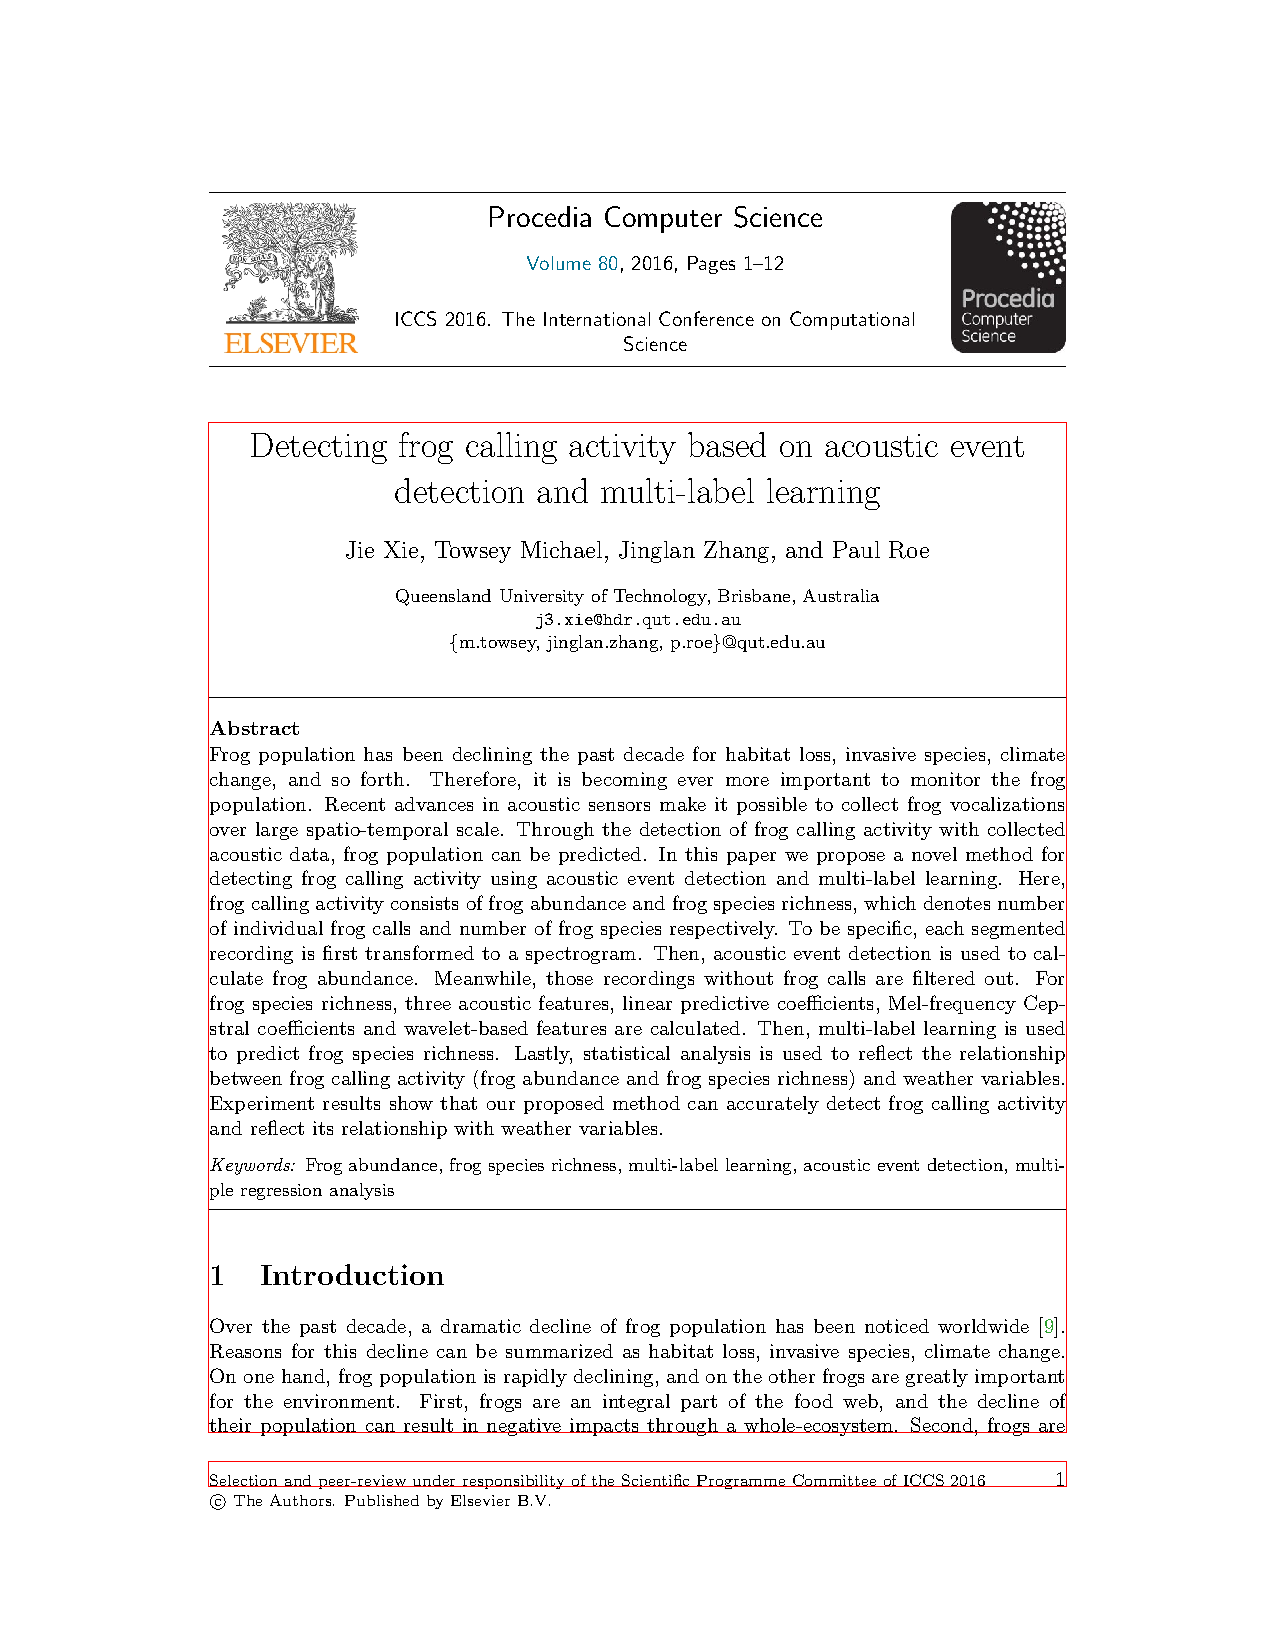
\includepdf[pages=-, pagecommand={},width=1.5\textwidth]{Ch7_paper.pdf}

